\documentclass{article}
\usepackage{cmap}
\usepackage[utf8]{inputenc}
\usepackage[russian]{babel}
\usepackage{setspace,amsmath}
\usepackage{lipsum}
\usepackage[usestackEOL]{stackengine}
\usepackage{lipsum}
\usepackage{kantlipsum}
\usepackage[left=2cm,right=2cm,top=2cm,bottom=2cm,bindingoffset=0cm]{geometry}
\usepackage[pdftex]{graphicx}
\usepackage{lastpage}
\usepackage{titling}
\graphicspath{{pictures/}}
\DeclareGraphicsExtensions{.pdf,.png,.jpg}
\newcommand\zz[1]{\par{\normalsize\strut #1} \hfill\ignorespaces}
\addto\captionsrussian{\def\refname{Список использованных источников}}
\newcommand{\subtitle}[1]{%
  \posttitle{%
    \par\end{center}
    \begin{center}\Large#1\end{center}
   }%
}
\newcommand{\subsubtitle}[1]{%
  \preauthor{%
    \begin{center}
    \large #1 \vskip0.5em
    \begin{tabular}[t]{c}
    }%
}
\begin{document}
 
\begin{center}
\textbf{
ПРАВИТЕЛЬСТВО РОССИЙСКОЙ ФЕДЕРАЦИИ\\
НАЦИОНАЛЬНЫЙ ИССЛЕДОВАТЕЛЬСКИЙ УНИВЕРСИТЕТ\\
«ВЫСШАЯ ШКОЛА ЭКОНОМИКИ»\\
Факультет компьютерных наук
Образовательная программа «Программная инженерия»\\
(ВШЭ ФКН ПИ)}\\
\end{center}
УДК 004.852
\bigskip
\zz{~}УТВЕРЖДАЮ
\zz{~}Академический руководитель
\zz{~}образовательной программы
\zz{~}«Программная инженерия»
\zz{~}профессор департамента программной
\zz{~}инженерии, канд. техн. наук
\zz{~}\noindent\rule{3cm}{0.4pt} В.В. Шилов
\zz{~}«\noindent\rule{1cm}{0.4pt}»\noindent\rule{2cm}{0.4pt}20\noindent\rule{0.5cm}{0.4pt}г.
\begin{center}
\topskip=0pt
\vspace*{\fill}
\textbf{ОТЧЕТ\\
О НАУЧНО-ИССЛЕДОВАТЕЛЬСКОЙ РАБОТЕ}\\
~\\
ОБУЧЕНИЕ С ПОДКРЕПЛЕНИЕМ ДЛЯ ЗАДАЧ РАСПРЕДЕЛЕНИЯ РЕСУРСОВ В ОБЛАКЕ\\
(заключительный)\\
\vspace*{\fill}
\end{center}
\zz{Руководитель НИР:}Выполнил:
\zz{Приглашенный лектор,}Студент группы БПИ204
\zz{главный инженер Huawei}образовательной программы
\zz{~}«Программная инженерия»
\zz{Андрей Александрович Тихонов}Пеганов Никита Сергеевич
\zz{\noindent\rule{3cm}{0.4pt} А. А. Тихонов}\noindent\rule{3cm}{0.4pt} Н. С. Пеганов
\zz{«\noindent\rule{1cm}{0.4pt}»\noindent\rule{2cm}{0.4pt}20\noindent\rule{0.5cm}{0.4pt}г.}«\noindent\rule{1cm}{0.4pt}»\noindent\rule{2cm}{0.4pt}20\noindent\rule{0.5cm}{0.4pt}г.
\begin{center}
\vspace*{\fill}{
  Москва 2022}
\end{center}
\newpage
\begin{center}
\section {Реферат}
\end{center}
Отчет \pageref{LastPage} с., 1 кн., 4 рис., 2 табл., 19 источн., 1 прил.
\bigskip
ОБУЧЕНИЕ С ПОДКРЕПЛЕНИЕМ, REINFORCEMENT LEARNING, RL, РАСПРЕДЕЛЕНИЕ РЕСУРСОВ В ОБЛАКЕ, ОБЛАЧНЫЕ ТЕХНОЛОГИИ, ОБЛАЧНЫЕ РЕСУРСЫ, TETRIS, OPENAI GYM, TENSORFLOW, KERASRL
\bigskip
Объектом исследования являются особенности выделения ресурсов при работе с облачными сервисами.
\bigskip
Целью работы является исследование применимости обучения с подкреплением в задачах распределения облачных ресурсов, а также сравнение данного подхода с другими методами решения задачи. 
\bigskip
В ходе работы проведен пробный эксперимент для изучения используемого метода — автоматическая игра в Тетрис. Также проведены экспериментальные исследования выбранного метода решения задачи.
\bigskip
В процессе изучения иных работ было выяснено, что обучение с подкреплением примянялось в решении задачи распределения данных в облаке, но данная область не является достаточно изученной.
\bigskip
В результате проведенного исследования было выяснено, что выбранный мной способ не является применимым при решении данной задачи или требует дальнейших исследований.
\bigskip
Исследование показало, что выбранный мной способ решения задачи не позволяет улучшить взятые для анализа метрики.\\
\bigskip
Исходя из полученных результатов, можно предположить, что для улучшения полученных метрик возможно использовать другие виды машинного обучения.
\newpage
\begin{center}
\section {Содержание}
\tableofcontents
\end{center}
\newpage
\section {Основные термины, определения и сокращения}
Внастоящем отчете о НИР применяютследующиесокращения и обозначения.
\bigskip
CPU (англ. central processing unit) — электронное устройство, исполняющее машинный код программ, главная часть аппаратного обеспечения компьютера. Иногда также называется микропроцессором или процессором
\bigskip
IT (произносится ай-ти, сокращение от англ. Information Technology) — информационные технологии
\bigskip
RAM (англ. Random Access Memory) — запоминающее устройство с произвольным доступом, один из видов памяти компьютера, позволяющий единовременно получить доступ к любой ячейке по её адресу на чтение или запись
\bigskip
RL (англ. reinforcement learning) — обучение с подкреплением
\bigskip
Облачные технологии — IT-технологии, которые позволяют хранить и обрабатывать информацию на удалённых от клиента серверах
\bigskip
Облако — набор из некоторого количества IT-ресурсов, размещенных в инфраструктуре облачного провайдера
\bigskip
Обучение с подкреплением (англ. reinforcement learning) — один из видов машинного обучения, в ходе применения которого испытуемая система, называемая агентом, обучается, взаимодействуя со средой
\bigskip
\newpage
\begin{center}
\section {Введение}
\end{center}
В первой части работы описано применение обучения с подкреплением для обучения агента самостоятельному прохождению в компьютерной игры Тетрис\cite{litlink1}. Эта игра представляет собой клетчатое поле шириной 10 клеток и высотой 20 клеток. В верхней части поля друг за другом появляются клетчатые фигурки, состоящие из 4 клеток (тетрамино). Фигурки имеют форму, напоминающую форму букв "I", "Z", "L", "T", а также квадрат из четырех клеток. Пользователь имеет возможность поворачивать фигурку на 90°, а также двигать ее по горизонтали во время падения. В случае заполнения одной из строк частями фигурок строка "исчезает": все фигурки выше нее опускаются на одну строку вниз. Каждая "исчезнувшая" строка приносит игроку 1 очко.
Во второй части работы обучение с подкреплением применено для решения задач распределения облачных ресурсов.\\
\textbf{Актуальность}\\
Облачные технологии позволяют обеспечить круглосуточную и бесперебойную работу интернет-сервисов, что делает их востребованными во всех сферах IT-индустрии. Облачными вычислениями занимаются Amazon, Google, Huawei и другие крупнейшие информационные компании\cite{litlink2}\cite{litlink3}. В 2020 году мировой рынок облачных вычислений оценивается в 289.25 миллиардов долларов\cite{litlink4}. Распределение облачных ресурсов — одна из важнейших задач облачных вычислений.\\
\textbf{Предмет исследования}\\
Возможность использования обучения с подкреплением для решения задачи распределения ресурсов облака.\\
\textbf{Методы исследования}\\
Экспериментальное сравнение показателей RL в ходе решения задачи распределения облачных ресурсов с иными используемыми на практике способами. Для наглядности в работе также решена близкая задача: автоматическая игра в "Тетрис" с помощью обучения с подкреплением.  Данная компьютерная игра выбрана неслучайно: она имеет концепции, сходные с основной задачей. Во-первых, ее основная цель — упаковка фигур. В решаемой задаче так же требуется распределять задачи пользователей между имеющимися ресурсами серверов. Во-вторых, игра имеет два параметра — координаты X и Y. Основная задача так же имеет два параметра, которые требуется распределять: CPU и RAM. Также решение задачи автоматической игры в "Тетрис" позволила научиться применять использованные библиотеки и фреймворки на практике.\\
\textbf{Цели и задачи работы}\\
Определение эффективность обучения с подкреплением в задаче распределения ресурсов в облаке.\\
\textbf{Новизна и достоверность полученных результатов}
Данная исследовательская работа не является первой работой, написанной на данную тему, однако, RL пока не было применено на практике для решения исследуемой задачи. Это показывает, что данная область нуждается в изучении.\\
\textbf{Теоретическая значимость}\\
Работа не имеет теоретической значимости, так как опирается на уже исследованный алгоритм обучения с подкреплением.\\
\textbf{Практическая ценность}\\
В случае превосходства RL над другими методами в рамках решения задачи распределения облачных ресурсов применение данного способа машинного обучения способно сократить нагрузку на сервера, предоставляющие доступ к облачным сервисам. Это позволит уменьшить расходы компаний на поддержку их работоспособности, а также расходы на производство при сокращении количества серверов. Проект имеет практическую ценность для экологии: уменьшение расходов электроэнергии приведет к уменьшению углеродного следа компаниий.	\\
\newpage
\begin{center}
\section {Основная часть отчёта о НИР}
\end{center}
\begin{center}
\item\subsection{Применение обучения с подкреплением в игре «Тетрис»}
\end{center}
Первая часть курсовой работы посвящена автоматической игре в "Тетрис" с помощью обучения с подкреплением. Рассмотрим исследования данной задачи и ее решения. В статье "Tetris is Hard, Even to Approximate"\cite{litlink6} доказывается, что игра Тетрис является NP-полной задачей. Это одна из причин схожести данной игры с распределением ресурсов в облаке\cite{litlink6}. В статье Playing the Original Game Boy Tetris Using a Real Coded Genetic Algorithm\cite{litlink7} используется генетический алгоритм для симуляции игры в тетрис. В данной работе метриками успеха автор считает максимальное число удаленных строк до поражения и среднее число удаленных строк у запущенного несколько раз алгоритма. Обе метрики значительно уступают роевым оптимизациям,  продемонстрированным в работах Apply ant colony optimization to tetris\cite{litlink19} и Swarm tetris: Applying particle swarm optimization to tetris\cite{litlink10}. Примером использования RL для игры в Тетрис является статья A deep reinforcement learning bot that plays tetris\cite{litlink13}.\\~\\
Таким образом, исследование источников показало, что обучение с подкреплением активно используется для решения задачи автоматической игры в "Тетрис". Это объясняется тем, что "Тетрис" — дискретная задача, и в ней есть четкое разделение между средой и агентом. Средой выступает клетчатое поле, которое заполняется фигурами в процессе игры, а агентом является "игрок", двигающий фигуры влево и вправо. При этом агент взаимодействует со средой, расставляя на поле фигуры, а среда возвращает агенту количество удаленных строк и расположение поставленных фигур на поле.\\~\\
Для демонстрации работы обучения с подкреплением на примере игры "Тетрис" требовалось выбрать среду для симуляции игры, а также библиотеку для реализации машинного обучения. 
В качестве среды был рассмотрен симулятор устройства для игр "Game Boy"\ PyBoy\cite{litlink3}. Однако он был отвергнут в пользу более популярной и более простой в использовании библиотеки gym-tetris\cite{litlink5}, являющейся частью OpenAI Gym\cite{litlink14} — среды для симуляции известных компьютерных игр и физических задач.\\
При выборе библиотеки были рассмотрены pyqlearning\cite{litlink1} и Tensorforce\cite{litlink17}. Однако выбрана была библиотека KerasRL\cite{litlink9}, надстройка над фреймворком TensorFlow\cite{litlink16}. Выбор был сделан в пользу KerasRL из-за совместимости со средой OpenAI Gym.\\
В игре "Тетрис" могут быть использованы различные метрики для рассчета награды агента. Например, число убранных строк, количество сброшенных фигурок, число ходов до проигрыша, переход на новую скорость и другие. Для простоты в качестве награды было выбрано число убранных строк.\\~\\
Рассмотрим библиотеки, выбранные для решения поставленной задачи. Библиотека OpenAI Gym применяется для обучения нейронных сетей игре в различные компьютерные игры, а также решения физических задач таких, как хождение и удержание баланса. \\
TensorFlow — фреймворк с открытым кодом, совмещающий в себе передовые достижения для создания и использования нейронных сетей. Библиотека создана компанией Google, однако активно развивается сообществом программистов\cite{litlink18}.\\
Библиотека KerasRL позволяет создать нейронную сеть и агента, который будет взаимодействовать со средой и обучать сеть. Библиотека также является открытой и развивается компанией Google.\\~\\
Для решения поставленной задачи выбран метод обучения с подкреплением. Это способ машинного обучения, при котором система, называемая агентом, обучается во время взимодействия со средой (в первой части работы средой является компьютерная игра "Тетрис"). При этом агент влияет на среду с помощью действий, а среда взаимодействует с агентом, показывая ему информацию о состоянии среды, а также возвращая награду. Цель агента — максимизация награды.\\
\begin{figure}[h]
\center{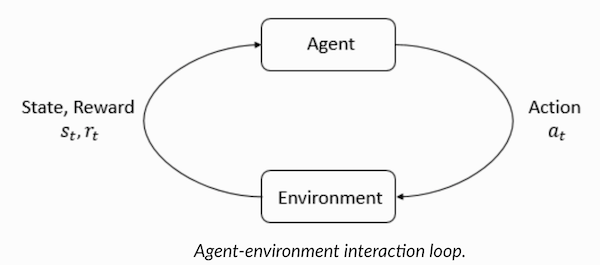
\includegraphics[width=1\linewidth]{RL_scheme}}
\caption{Схема метода обучения с подкреплением\cite{litlink19}.}
\label{ris:image}
\end{figure}
\newpage
В первую очередь, с помощью библиотеки OpenAI Gym была создана среда, в которой обучающийся агент производит какие-либо действия. В случае, рассматриваемом в данной работе, создается среда TetrisA-v0 — эмулятор игры "Тетрис". В этой среде агент может сделать ход, передав один из вариантов действий: сдвиг фигурки влево, сдвиг фигурки вправо, поворот на 90° по часовой стрелке, против часовой стрелки, ускорение падения фигурки. При заполнении строки частями фигурок среда автоматически очищает строку и добавляет 1 к награде.\\
\begin{figure}[h]
\center{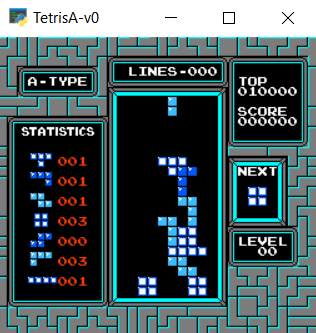
\includegraphics[width=\linewidth/3]{tetris_example}}
\caption{Пример среды TetrisA-v0.}
\label{ris:image}
\end{figure}\\
\newpage
Затем с помощью библиотеки KerasRL была создана модель нейронной сети со следующими слоями. 1 слой, необходимый для сглаживания входных данных. Входными данными является информация, занята или свободна каждая клетка игрового поля. 2 сильно связанный слой с 24 входными синапсами и функцией активации выпрямленного линейного блока. Последний сильно связанный слой имеет линейную функцию активации и 12 выходных синапсов: каждый синапс отвечает за одно из действий.\\
\begin{figure}[h]
\center{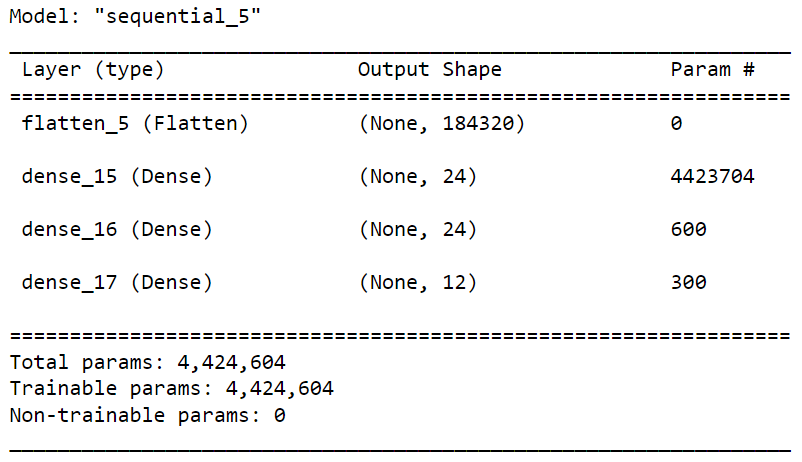
\includegraphics[width=\linewidth/2]{network}}
\caption{Краткое описание нейронной сети.}
\label{ris:image}
\end{figure}\\
На основе данной сети был создан агент с политикой BoltzmannQPolicy. Это означает, что агент вычисляет вид распределения значений, возвращаемых средой, и выбирает случайное действие на основе этого распределения.\\
После 50000 шагов, занявших 8 часов 11 минут, агент научился играть в "Тетрис" со среднем значением награды 11.02. При этом среднее число шагов до проигрыша было равно 4260.23.\\~\\
Сравним полученный результат с другими реализациями RL в игре Tetris. В статье Playing the Original Game Boy Tetris Using a Real Coded Genetic Algorithm\cite{litlink7} средний результат алгоритма "FS-B" составил 30.71 ± 15.82, что является сравнимым с полученным значением. В работе Learn to Play Tetris with Deep Reinforcement Learning\cite{litlink20} алгоритмы Dreamer, Plan2xplore и LucidDreamer получили 55, 72 и 107 значений стертых линий, что является большим, но близким к полученному результатом. Таким образом, эксперимент с автоматической игрой в "Тетрис" показал, что RL является применимым к данной задаче алгоритмом и получает значимый результат.
\newpage
\begin{center}
\item\subsection{Применение обучения с подкреплением в основной задаче}
\end{center}
\newpage
\begin{center}
\section {Заключение}
\end{center}
\newpage
\begin{center}
\begin{thebibliography}{}
\bibitem{litlink1}  \textit{Kent, Steven} (2001) The Ultimate History of Video Games: From Pong to Pokemon: The Story Behind the Craze That Touched Our Lives and Changed the World (1st ed.). Three Rivers Press. С. 377-381. 
    \bibitem{litlink2}  \textit{Arif Mohamed} (2018) A history of cloud computing // Сайт Сomputerweekly.com. 9 апреля (https://www.computerweekly.com/feature/A-history-of-cloud-computing) Просмотрено: 11.12.2021.
    \bibitem{litlink3}  \textit{Matt Kapko} (2021) Can Huawei ‘Reinvent Itself’ as a Cloud Leader? // Сайт Sdxcentral.com. 26 апреля (https://www.sdxcentral.com/articles/news/can-huawei-reinvent-itself-as-a-cloud-leader/2021/04/) Просмотрено: 11.12.2021
    \bibitem{litlink4} \textit{Laura Wood} (2021) Global Cloud Computing Market (2020 to 2026) - by Service, Deployment, Application Type, End-user and Region Businesswire.com. 24 августа (https://www.businesswire.com/news/home/20210824005585/en/Global-Cloud-Computing-Market-2020-to-2026---by-Service-Deployment-Application-Type-End-user-and-Region---ResearchAndMarkets.com) Просмотрено: 11.12.2021
\bibitem{litlink5}  \textit{Erik D. Demaine, Susan Hohenberger, David Liben-Nowell} (2002) Tetris is Hard, Even to Approximate // Сайт Arxiv.org. 21 октября (https://arxiv.org/abs/cs/0210020) Просмотрено: 11.12.2021
\bibitem{litlink6}  \textit{Harvinder Singh, Anshu Bhasin, Parag Ravikant Kaveri} (2021) QRAS: efficient resource allocation for task scheduling in cloud computing // Сайт Researchgate.net. Апрель (https://www.researchgate.net/publication/350192028\_QRAS\_efficient\_resource\_allocation\_for\_task\_\\scheduling\_in\_cloud\_computing) Просмотрено: 11.12.2021
\bibitem{litlink7} \textit{Renan Samuel da Silva, Rafael Stubs Parpinelli} (2017) Playing the Original Game Boy Tetris Using a Real Coded Genetic Algorithm // Сайт Researchgate.net. Октрябрь (https://www.researchgate.net/publication/322321608\_Playing\_the\_Original\_Game\_Boy\_Tetris\_Using\_a\_\\Real\_Coded\_Genetic\_Algorithm) Просмотрено: 11.12.2021
\bibitem{litlink8} \textit{X. Chen, H. Wang, W. Wang, Y. Shi, and Y. Gao} (2009) Apply ant colony optimization to tetris // Сайт Dl.acm.org. 8 июля (https://dl.acm.org/doi/10.1145/1569901.1570136) Просмотрено: 11.12.2021
\bibitem{litlink9} \textit{L. Langenhoven, W. S. van Heerden, and A. P. Engelbrecht} (2010) Swarm tetris: Applying particle swarm optimization to tetris // Сайт Ieeexplore.ieee.org. 18-23 июля (https://ieeexplore.ieee.org/document/5586033) Просмотрено: 11.12.2021
\bibitem{litlink10} \textit{nuno-faria, nlinker (Nick Linker)} (2019) A bot that plays tetris using deep reinforcement learning. // Сайт Github.com. 7 сентября (https://github.com/nuno-faria/tetris-ai) Просмотрено: 11.12.2021
\bibitem{litlink11} \textit{Baekalfen (Mads Ynddal)} (2021) Game Boy emulator written in Python. // Сайт Github.com. 22 октября (https://github.com/Baekalfen/PyBoy) Просмотрено: 01.02.2022
\bibitem{litlink12} \textit{Christian Kauten} (2019) An OpenAI Gym environment for Tetris on The Nintendo Entertainment System (NES) based on the nes-py emulator. // Сайт Pypi.org. 3 июня (https://github.com/Baekalfen/PyBoy) Просмотрено: 01.02.2022
\bibitem{litlink13} \textit{OpenAI} (2021) A toolkit for developing and comparing reinforcement learning algorithms. // Сайт Github.com. 2 октября (https://github.com/openai/gym) Просмотрено: 01.02.2022
\bibitem{litlink14} \textit{accel-brain, chimera0} (2020) Reinforcement Learning Library: pyqlearning. // Сайт Pypi.org. 13 июля (https://pypi.org/project/pyqlearning/) Просмотрено: 01.02.2022
\bibitem{litlink15} \textit{Tensorforce} (2021) Tensorforce: a TensorFlow library for applied reinforcement learning. // Сайт Github.com. 30 августа (https://github.com/tensorforce/tensorforce) Просмотрено: 01.02.2022
\bibitem{litlink16} \textit{Keras-RL} (2018) Deep Reinforcement Learning for Keras. // Сайт Github.com. 1 мая (https://github.com/keras-rl/keras-rl) Просмотрено: 01.02.2022
\bibitem{litlink17} \textit{tensorflow} (2021) An Open Source Machine Learning Framework for Everyone. // Сайт Github.com. 4 ноября (https://github.com/tensorflow/tensorflow) Просмотрено: 01.02.2022
\bibitem{litlink18} \textit{Cade Metz} (2015) TensorFlow, Google's Open Source AI, Signals Big Changes in Hardware Too. // Сайт Wired.com. 10 ноября (https://www.wired.com/2015/11/googles-open-source-ai-tensorflow-signals-fast-changing-hardware-world/) Просмотрено: 02.02.2022
\bibitem{litlink19} \textit{Vihar Kurama, Samhita Alla} (2018) Обучение с подкреплением на языке Python. // Сайт Habr.com. 28 декабря (https://habr.com/ru/company/piter/blog/434738/) Просмотрено: 02.02.2022
\bibitem{litlink20} \textit{Hanyuan Liu, Lixin Liu} (2020) Learn to Play Tetris with Deep Reinforcement Learning. // Сайт Openreview.net. 14 декабря (https://openreview.net/forum?id=8TLyqLGQ7Tg) Просмотрено: 05.05.2022
\end{thebibliography}
\end{center}
\newpage
\begin{center}
\section {Приложения}
\end{center}
\zz{}\textbf{Приложение 1\\}
Ссылка на репозиторий проекта с исходным кодом и всеми использованными материалами.\\
https://github.com/NikPeg/Reinforcement-learning-for-resource-allocation-tasks-in-the-cloud
\end{document}